
\chapter{Image Fusion }\label{sec:Fusion}
%\section{Introduction}

Satellite sensors present an important diversity in terms of characteristics.
Some provide a high spatial resolution while other focus on providing several
spectral bands. The fusion process brings the information from different
sensors with different characteristics together to get the best of both
worlds.

Most of the fusion methods in the remote sensing community deal with
the {\em pansharpening technique}. This fusion combines the image from
the PANchromatic sensor of one satellite (high spatial resolution
data) with the multispectral (XS) data (lower resolution in several
spectral bands) to generate images with a high resolution and several
spectral bands. Several advantages make this situation easier:

\begin{itemize}
\item PAN and XS images are taken simultaneously from the same satellite (or
with a very short delay);
\item the imaged area is common to both scenes;
\item many satellites provide these data (SPOT 1-5, Quickbird, Pleiades)
\end{itemize}

This case is well-studied in the literature and many methods exist. Only very
few are available in OTB now but this should evolve soon.


\section{Simple Pan Sharpening}\label{secPanSharpening}

A simple way to view the pan-sharpening of data is to consider that,
at the same resolution,  the panchromatic channel is the sum of the XS
channel. After putting the two images in the same geometry, after
orthorectification (see chapter \ref{sec:Ortho}) with an oversampling of the XS image, we can proceed to the data fusion. 

The idea is to apply a low pass filter to the panchromatic band to give it a spectral content (in the Fourier domain) equivalent to the XS data. Then we normalize the XS data with this low-pass panchromatic and multiply the result with the original panchromatic band.

The process is described on figure \ref{fig:PanSharpening}.

\begin{figure}[th]
  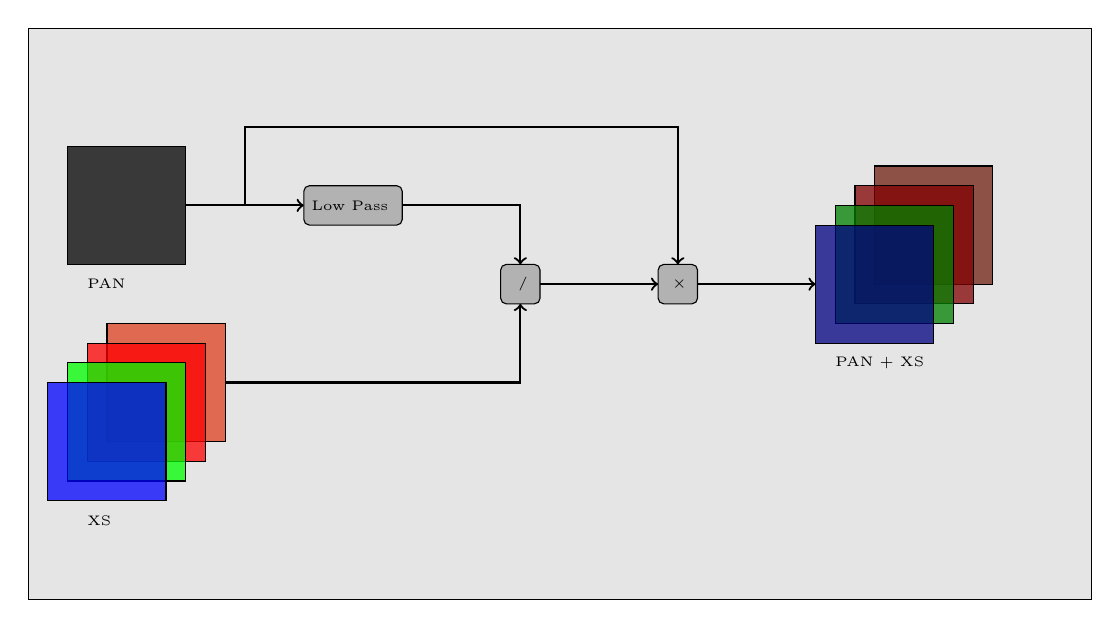
\begin{tikzpicture}[scale=0.25]
    \tiny
    \draw[fill=black!10] (-1,-12) rectangle (53,17);
	\filldraw[fill=red!50!brown,fill opacity=0.75] (3,-4) rectangle +(6,6);
	\filldraw[fill=red,fill opacity=0.75] (2,-5) rectangle +(6,6);
	\filldraw[fill=green,fill opacity=0.75] (1,-6) rectangle +(6,6);
	\filldraw[fill=blue,fill opacity=0.75] (0,-7) rectangle +(6,6);
	\node[anchor=center, text width= 1cm] (XS) at (4,-8) {XS};
	\filldraw[fill=black,fill opacity=0.75] (1,5) rectangle +(6,6);
	\node[anchor=center, text width= 1cm] (PAN) at (4,4) {PAN};

	\draw[->,thick] (7,8) --  +(6,0);

	\draw[fill=black!30,rounded corners=2pt] (13,7) rectangle +(5,2);
	\node[text width= 1.3cm] (Lowpass) at (16,8) {Low Pass};

	\draw[->,thick] (18,8) --  ++(6,0) -- ++(0,-3);
	\draw[->,thick] (9,-1) --  ++(15,0) -- ++(0,4);

	\draw[fill=black!30,rounded corners=2pt] (23,3) rectangle +(2,2);
	\node[text width= 1.3cm] (Div) at (26.5,4) {/};

	\draw[->,thick] (25,4) --  ++(6,0);
	\draw[->,thick] (10,8) --  ++(0,4) -- ++(22,0) -- ++(0,-7);

	\draw[fill=black!30,rounded corners=2pt] (31,3) rectangle +(2,2);
	\node[anchor=center, text width= 1cm] (Mult) at (33.7,4) {$\times$};

	\draw[->,thick] (33,4) --  ++(6,0);

	\filldraw[fill=red!50!brown!50!black,fill opacity=0.75] (42,4) rectangle +(6,6);
	\filldraw[fill=red!50!black,fill opacity=0.75] (41,3) rectangle +(6,6);
	\filldraw[fill=green!50!black,fill opacity=0.75] (40,2) rectangle +(6,6);
	\filldraw[fill=blue!50!black,fill opacity=0.75] (39,1) rectangle +(6,6);
	\node[anchor=center, text width= 2cm] (PANXS) at (44,0) {PAN + XS};

  \end{tikzpicture}

\itkcaption[Simple pan-sharpening]{Simple pan-sharpening procedure.}
\label{fig:PanSharpening}
\end{figure}

\input{PanSharpeningExample.tex}

\section{Bayesian Data Fusion}\label{secBayesian}


\input{BayesianFusionImageFilter.tex}
